\documentclass[12pt]{article}
	
%______________________PREAMBULO_________________________

%----------------------Paquetes--------------------------
\usepackage{amsmath,amssymb,amsfonts,latexsym,cancel} % Paquetes de símbolos adicionales.
\usepackage[spanish,es-tabla]{babel} % Idioma español
\usepackage[utf8]{inputenc} % Paquete que nos permite usar los acentos y otros símbolos, directamente del teclado.
\usepackage[T1]{fontenc} % Cambia el tipo de letra
\usepackage{times} % Tipo de letra Times New Roman
\usepackage{graphicx} % Paquete para el manejo de gráficos y figuras en el documento.
\usepackage{geometry} % Permite el manejo de los margenes
\usepackage{fancyhdr} % Permite colocar y manejar el encabezado
\usepackage[breaklinks,colorlinks=true,linkcolor=black,citecolor=blue, urlcolor=blue]{hyperref} % Crea hipervinculo entre secciones y el indice
\usepackage{pstricks}
\usepackage{multicol}
%\usepackage{mathpazo} %fuente palatino
%\usepackage{xcolor}
%\usepackage[shortlabels]{enumitem}
%-------------Paquetes para el formato de las citas-------
%\usepackage[hyphens]{url}
%\usepackage{float}
%\usepackage{cite}
%\usepackage{wrapfig}

%-----------------------------ayuda de paquetes--------------------

\spanishdecimal{.}

%------------------------Margenes----------------------------

\newgeometry{bottom = 2.5 cm, top = 2.5 cm, left = 2 cm, right = 2 cm} % Modifica el margen {Abajo, Arriba, Izquierda, Derecha

%----------------------------Interlineado----------------------------------

%\doublespacing
%\onehalfspace
%\singlespace
%\spacing{1.5} % Permite personalisar a gusto
%\setlength{\parskip}{2cm} % Es el espacio entre parrafos

%-----------------------------Sangria---------------------------------------

\setlength{\parindent}{0 cm} % Manipula la sangria

%---------------------Portada------------------

%\title{
%\begin{figure}[h!]
		
%	\centering
%	
\includegraphics[width=\linewidth]{Nom_UAdeC_FCFM.png}  			
			
%\end{figure}
%\huge \textbf{LABORATORIO DE FISICA 3}\\\LARGE TITULO PRACTICA\\}
%\author{ \Large \textbf{Profesor:}\\
%\Large \textbf{Alumno:} Oscar Joel Castro Contreras}
%\date{\today}

%--------------Encabezado y pie de pagina--------------------

\pagestyle{fancy}%Coloca el encabezado en el documento
\lhead[]{Métodos numéricos}%Encabezado izquierda
\rhead[]{Oscar Joel Castro Contreras}%Encabesado derecha
%\chead[]{}%Encabesado central
\renewcommand{\headrulewidth}{0.08 pt}%Coloca linea al pie de pagina

%\lfoot[]{PI}%Pie de pagina izquerdo
%\rfoot[]{PD}%Pie de pagina derecho
\cfoot[]{\thepage}%Pie de pagina central
\renewcommand{\footrulewidth}{0.08 pt}%Coloca linea al pie de pagina

%-----------------------------------------------------------------------------

	\begin{document}
		
		\begin{titlepage}
		
			\centering
			{\bfseries
			\begin{figure}[h!]
				\centering
				
\includegraphics[width=\linewidth]{Nom_UAdeC_FCFM.png} 				
			\end{figure}
			\par}
			\vspace{2cm}
			{\scshape\LARGE Métodos numéricos \par}
			\vspace{3cm}
			{\scshape\Huge \textbf{Método de la Regla falsa} \par}
			\vfill
			{\LARGE \textbf{Profesora:} Maria Guadalupe Godina Cubillo \par}
			\vspace{3cm}
			{\LARGE \textbf{Alumno:} Oscar Joel Castro Contreras \par}
			\vfill
			{\Large \today \par}
			\thispagestyle{empty}
			%\thispagestyle{fancy}
			
		\end{titlepage}
	
		\newpage

		\begin{abstract}
			\noindent En este reporte explico un poco de los métodos que existen para encontrar las raíces de cualquier 
			polinomio o función que tenga raíces, y en específico explico, qué es, en que consiste y cuales son las 
			limitaciones del método de la Regla falsa para encontrar raíces.
		\end{abstract}

		\textbf{Palabras clave:} Raíces, Regla falsa, Recta, Intervalo, Tolerancia.

		\section*{\centering Introducción}\label{sec:Introducción}
			Los polinomios son uno de los conceptos más importantes en álgebra y son fundamentales en 
			matemáticas y ciencia en general. Determinar las raíces de un polinomio es uno de los problemas 
			más antiguos en matemáticas.\\
			Puesto que las ecuaciones polinomiales aparecen en un amplio rango de áreas de la ciencia, desde 
			química y física básica hasta economía, el problema de determinar raíces de polinomios es, con 
			frecuencia, un paso obligado en la resolución de problemas.\cite{bib:item1}\\
			La razón principal para resolver ecuaciones no lineales por medio de métodos computacionales es 
			que algunas ecuaciones carecen de solución exacta, excepto por unas pocas. Por lo que existen 
			métodos numéricos diseñados para obtener las raíces, aunque cada uno tiene sus propias 
			limitaciones y defectos. Algunos métodos se muestran en la tabla \ref{tab:1}\cite{bib:item2}\\
			\begin{table}[h!]
				\centering
				\begin{tabular}{|c|c|}
					\hline
					\multicolumn{2}{|c|}{\textbf{Métodos numéricos para obtener raíces}}\\
					\hline
					\textbf{Nombre} & \textbf{Características} \\\hline
					Bisección & Aplicable a funciones no analiticas \\\hline
					Regla falsa & Convergencia lenta en un intervalo grande \\\hline								
					Método de Newton & Rápido, se nesecita calcular derivada \\\hline
					Método de secante & Rápido, no se requiera calcular derivada \\\hline
				\end{tabular}
				\caption{Métodos numéricos para obtener raíces \cite{bib:item2}}
				\label{tab:1}
			\end{table}\\
			En general, no es posible determinar los ceros de una función, es decir, valores $ x^* $ tal que $f(x^*) = 0 $, 
			en un número finito de pasos. Tenemos que usar métodos de aproximación. Los métodos son 
			usualmente iterativos y tienen la forma: Iniciando con una aproximación inicial $ x_0 $ (o un intervalo $ [a,b] $) , 
			se calculan aproximaciones sucesivas $ x_1,x_2,... $ y elegimos $ x_n $ como aproximación de $ x^* $ cuando se cumpla un 
			criterio de parada dado. A los ceros de un polinomio se les conoce también como raíces. \cite{bib:item3} \\
			\textbf{El método de la Regla falsa:}\\
			La falsa posición es una alternativa al método de bisección basada en evaluar $ f(x) $ en el 
			intervalo $ [a,b] $ y unir de $ f(a) $ y $ f(b) $ con una línea recta. La intersección de esta línea con 
			el eje de las x representa una mejor aproximación de la raíz. El hecho de que se reemplace la curva 
			por una línea recta da una “falsa posición” de la raíz; de aquí el nombre de método de la falsa 
			posición, o en latín, regula falsi. También se le conoce como método de la regla falsa.\\	
			Usando tiángulos semejante, la intersección de la recta con el eje x se estima mediante $$ \frac{f(a)}{c-a} = \frac{f(b)}{c-b} $$
			en la cual se depeja $ c $ $$ c = \frac{f(b)(a-b)}{f(a)-f(b)} $$ ésta es la fórmula de la regla falsa. El valor de $ c $ calculado, 
			reemplaza, despues, a cualquiera de los 2 valores iniciales, $ a $ o $ b $, y da un valor de la función con el mismo signo de $ f(c) $.
			De esta manera, los valores $ a $ y $ b $ simepre encierren la verdadera raíz. El proceso se repite hasta que la aproximación al raíz 
			sea adecuada. El algoritmo se parece al de bisección. \cite{bib:item4}

		\section*{\centering Metodología}\label{sec:Metodologia}
			El método consiste en suponer que tengamos un intervalo $ [a,b] $ donde esta una raíz de la función $ f(x) $. 
			Primero como en bisección evaluamos la función en los intervalos y verificamos $$ f(a)f(b) < 0 $$ 
			si esto no se cumple el método no funcionara para esa función, después de verificar que lo 
			anterior se cumple, debemos unir con una recta los puntos $ (a,f(a)) $ y $ (b,f(b)) $. Después se debe 
			encontrar el punto por el que la recta cruza el eje $ x $, para esto utilizamos la ecuación de la recta 
			$$ y_2-y_1 = m(x_2-x_1) $$ que en este caso sería $$ f(b)-f(a) = m (b-a) $$, entonces despejamos la 
			pendiente $$ m = \frac{f(b)-f(a)}{b-a} $$ y si suponemos que tenemos el punto que por el que cruza la recta 
			el eje $ x $ $ (c,0) $, entonces si hacemos un recta que cruce por el punto $ (c,0) $ y cualquiera 
			de los otros 2 puntos, tenemos la misma recta, por lo que ahora sustituimos en la ecuación de la 
			recta el punto $ (c,0) $, y cualquiera de los otros 2 punto anteriores, luego despejamos la pendiente y tenemos 
			que $$ m = \frac{0-f(b)}{c-b} $$, las pendiente la podemos igualar y despejar $ c $ $$ \frac{f(b)-f(a)}{b-a} = \frac{0-f(b)}{c-b} $$ 
			llegando a que $$ c = b-\frac{f(b)(b-a)}{f(b)-f(a)} $$ y como en bisección, en caso de que $ f(c) = 0 $, ya hemos 
			encontrado la raíz. Pero en caso de que no lo sea, ahora la raíz se encuentra entre $ [a,c] $ o $ [c,b] $. 
			para poder determinar a cuál de los 2 intervalos pertenece la raíz, hay que verificar $$ f(a)f(c) > 0 $$ 
			si esto se cumple, entonces, la raíz se encuentra en $ [a,c] $, si no se cumple ahora, hay que verificar 
			$$ f(b)f(c) > 0 $$ si esto se cumple, entonces, la raíz se encuentra en $ [c,b] $. Ahora repetimos todo el 
			proceso, pero con el intervalo nuevo obtenido. Así vamos iterando y reduciendo el intervalo las veces necesarias 
			para encontrar la mejor aproximación a la raíz de la función $ f(x) $.\\ 
			El criterio para parar las iteraciones es el mismo que bisección, está dado por el número de cifras 
			significativas que queramos, de aquí obtenemos una tolerancia, la cual en cada interacción se 
			compara con el error relativo y absoluto, si uno de los errores es menor o igual a la tolerancia, 
			detener las interacciones.\\
			El programa es casi idéntico que el de bisección lo único que cambia es la forma de obtener las 
			aproximaciones a la raíz, como ya obtuvimos la formula en el código estaría
			\begin{center}
				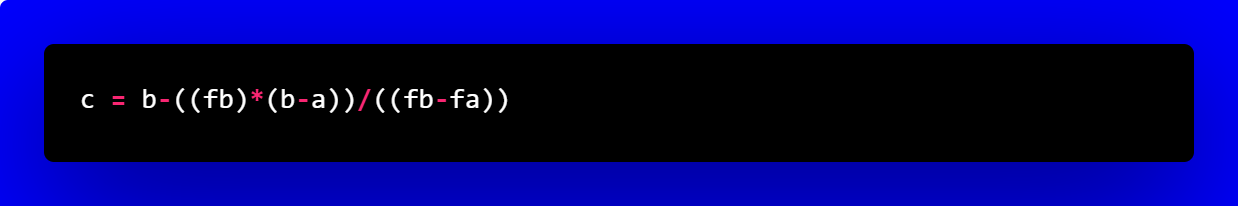
\includegraphics[width=\linewidth]{Figura 1.png} 
				Figura 1: Formula de aproximación a la raíz por el metodo de Regla falsa				
			\end{center}
	
		\section*{\centering Resultado}\label{sec:Resultado}
			Si tomamos el polinomio $ x^3-2x^2-1 $ y damos de intervalo inicial $ [1,3] $. Hacemos 
			la evaluación para obtener la raíz con 5 cifras significativas, el programa nos arroja
			\begin{multicols}{2}
				\begin{center}
					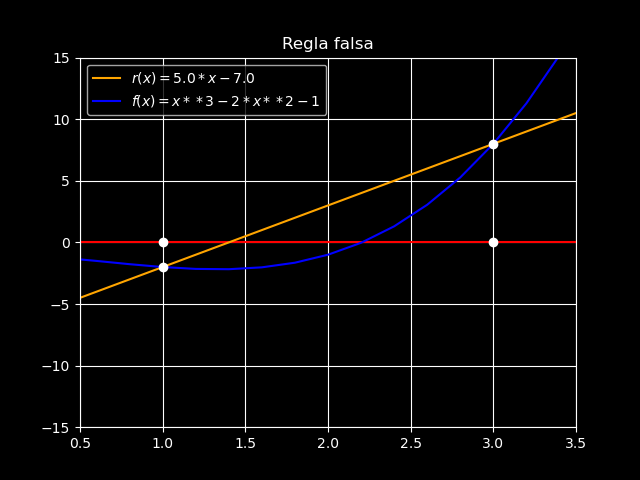
\includegraphics[width=\linewidth]{Grafica 1.png}
					Grafica 1: Recta que une los puntos obtenidos al evaluación el intervalo $ [1,3] $ en la función \columnbreak $ x^3-2x^2-1 $.\\
					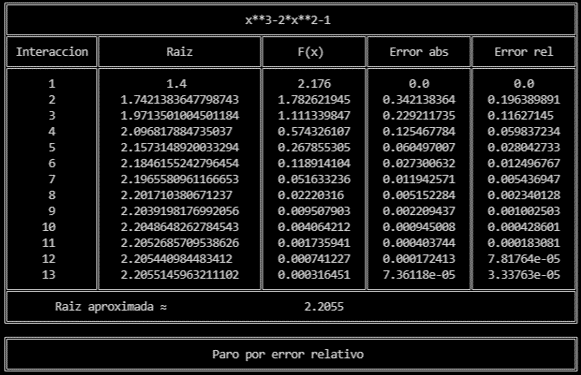
\includegraphics[width=\linewidth]{Tabla 1.png}
					Tabla 2: Iteraciones a la aproximación de la raíz de la función $ x^3-2x^2-1 $.
				\end{center}
			\end{multicols}
			Observamos que la aproximación a la raíz es $ 2.2055 $, con 13 iteraciones. El criterio de paro fue 
			por el error relativo.
		\section*{\centering Observación}\label{sec:Observacion}
			Como en bisección, si regresamos a la condición inicial de que $$ f(a)f(b) < 0 $$
			si esta condición no se cumple, el método no funciona para esa función, este es una de las 
			limitaciones del método, esto ocurre en diferentes situaciones.\\
			La condicion no se cumple cuando:
			\begin{itemize}
				\item En el intevalo $ [a,b] $, no hay la raícas, de la función.
				\item La funcion no tiene raíces reales,
				\item Hay mas de 1 raiz en el intervalo $ [a,b] $ dado.
				\item En general cuando la evaluación de $ f(a) $ tiene el mismo signo que $ f(b) $.
			\end{itemize}
		

		\section*{\centering Conclusión}\label{sec:Conclusion}
			En conclusión, el método de la regla falsa es muy similar al de bisección, con la diferencia que en 
			lugar de tomar el punto medio, se toma como nuevo valor la intersección con el eje $ x $ de un línea 
			recta formada por los 2 puntos del intervalo. Como en bisección esto solo se puede realizar si se 
			cumple que $ f(a)f(b) < 0 $.

		\centering
		\begin{thebibliography}{10}
			\bibitem{bib:item1} de la Vega, H. M. El calculo de raıces de polinomios. Una historia sin fin. Recuperado de
							\href{http://www.matedu.cinvestav.mx/~elcalculoysuensenanza/investigacion/articulosPDF/Madrid.pdf}{Pagina web de \cite{bib:item1}}.
			\bibitem{bib:item2} Nakamura, S. (1998). Metodos Numericos Aplicados Con Software. En Solución de ecuaciones no lineales (Primera ed., pp. 62–63). Prentice Hall.
			\bibitem{bib:item3} Mora, W. (2010). Introducción a los Métodos Numéricos. Implementaciones en R. Ecuaciones no lineales (Primera ed., pp. 95,110) Recuperado de
							\href{https://tecdigital.tec.ac.cr/revistamatematica/Libros/WMora_MetodosNumericos/2017_Principal_MetodosNumericos-con-R.pdf}{Pagina web de \cite{bib:item3}}. 
							\bibitem{bib:item4} Chapra, S. (2015). Métodos numéricos para ingenieros. RAICES DE ECUACIONES (7.a ed., pp. 91–180). Editorial McGraw-Hill.				
			
		\end{thebibliography}

	\end{document}